\section{The LAGO sites}\label{sec:sites}

As it was mentioned in previous sections, LAGO spans over many different
countries in Latin America. In this section we describe the sites according to
the location in each of the countries that have a LAGO detector. In
Fig.\ref{fig:lago-map}, a map of the Latin American region can be seen with the
sites marked where a LAGO WCD is in operation, to be installed in the 2014-2015
period or the sites in evaluation. Also the different countries are marke with
different colours.

\begin{figure}
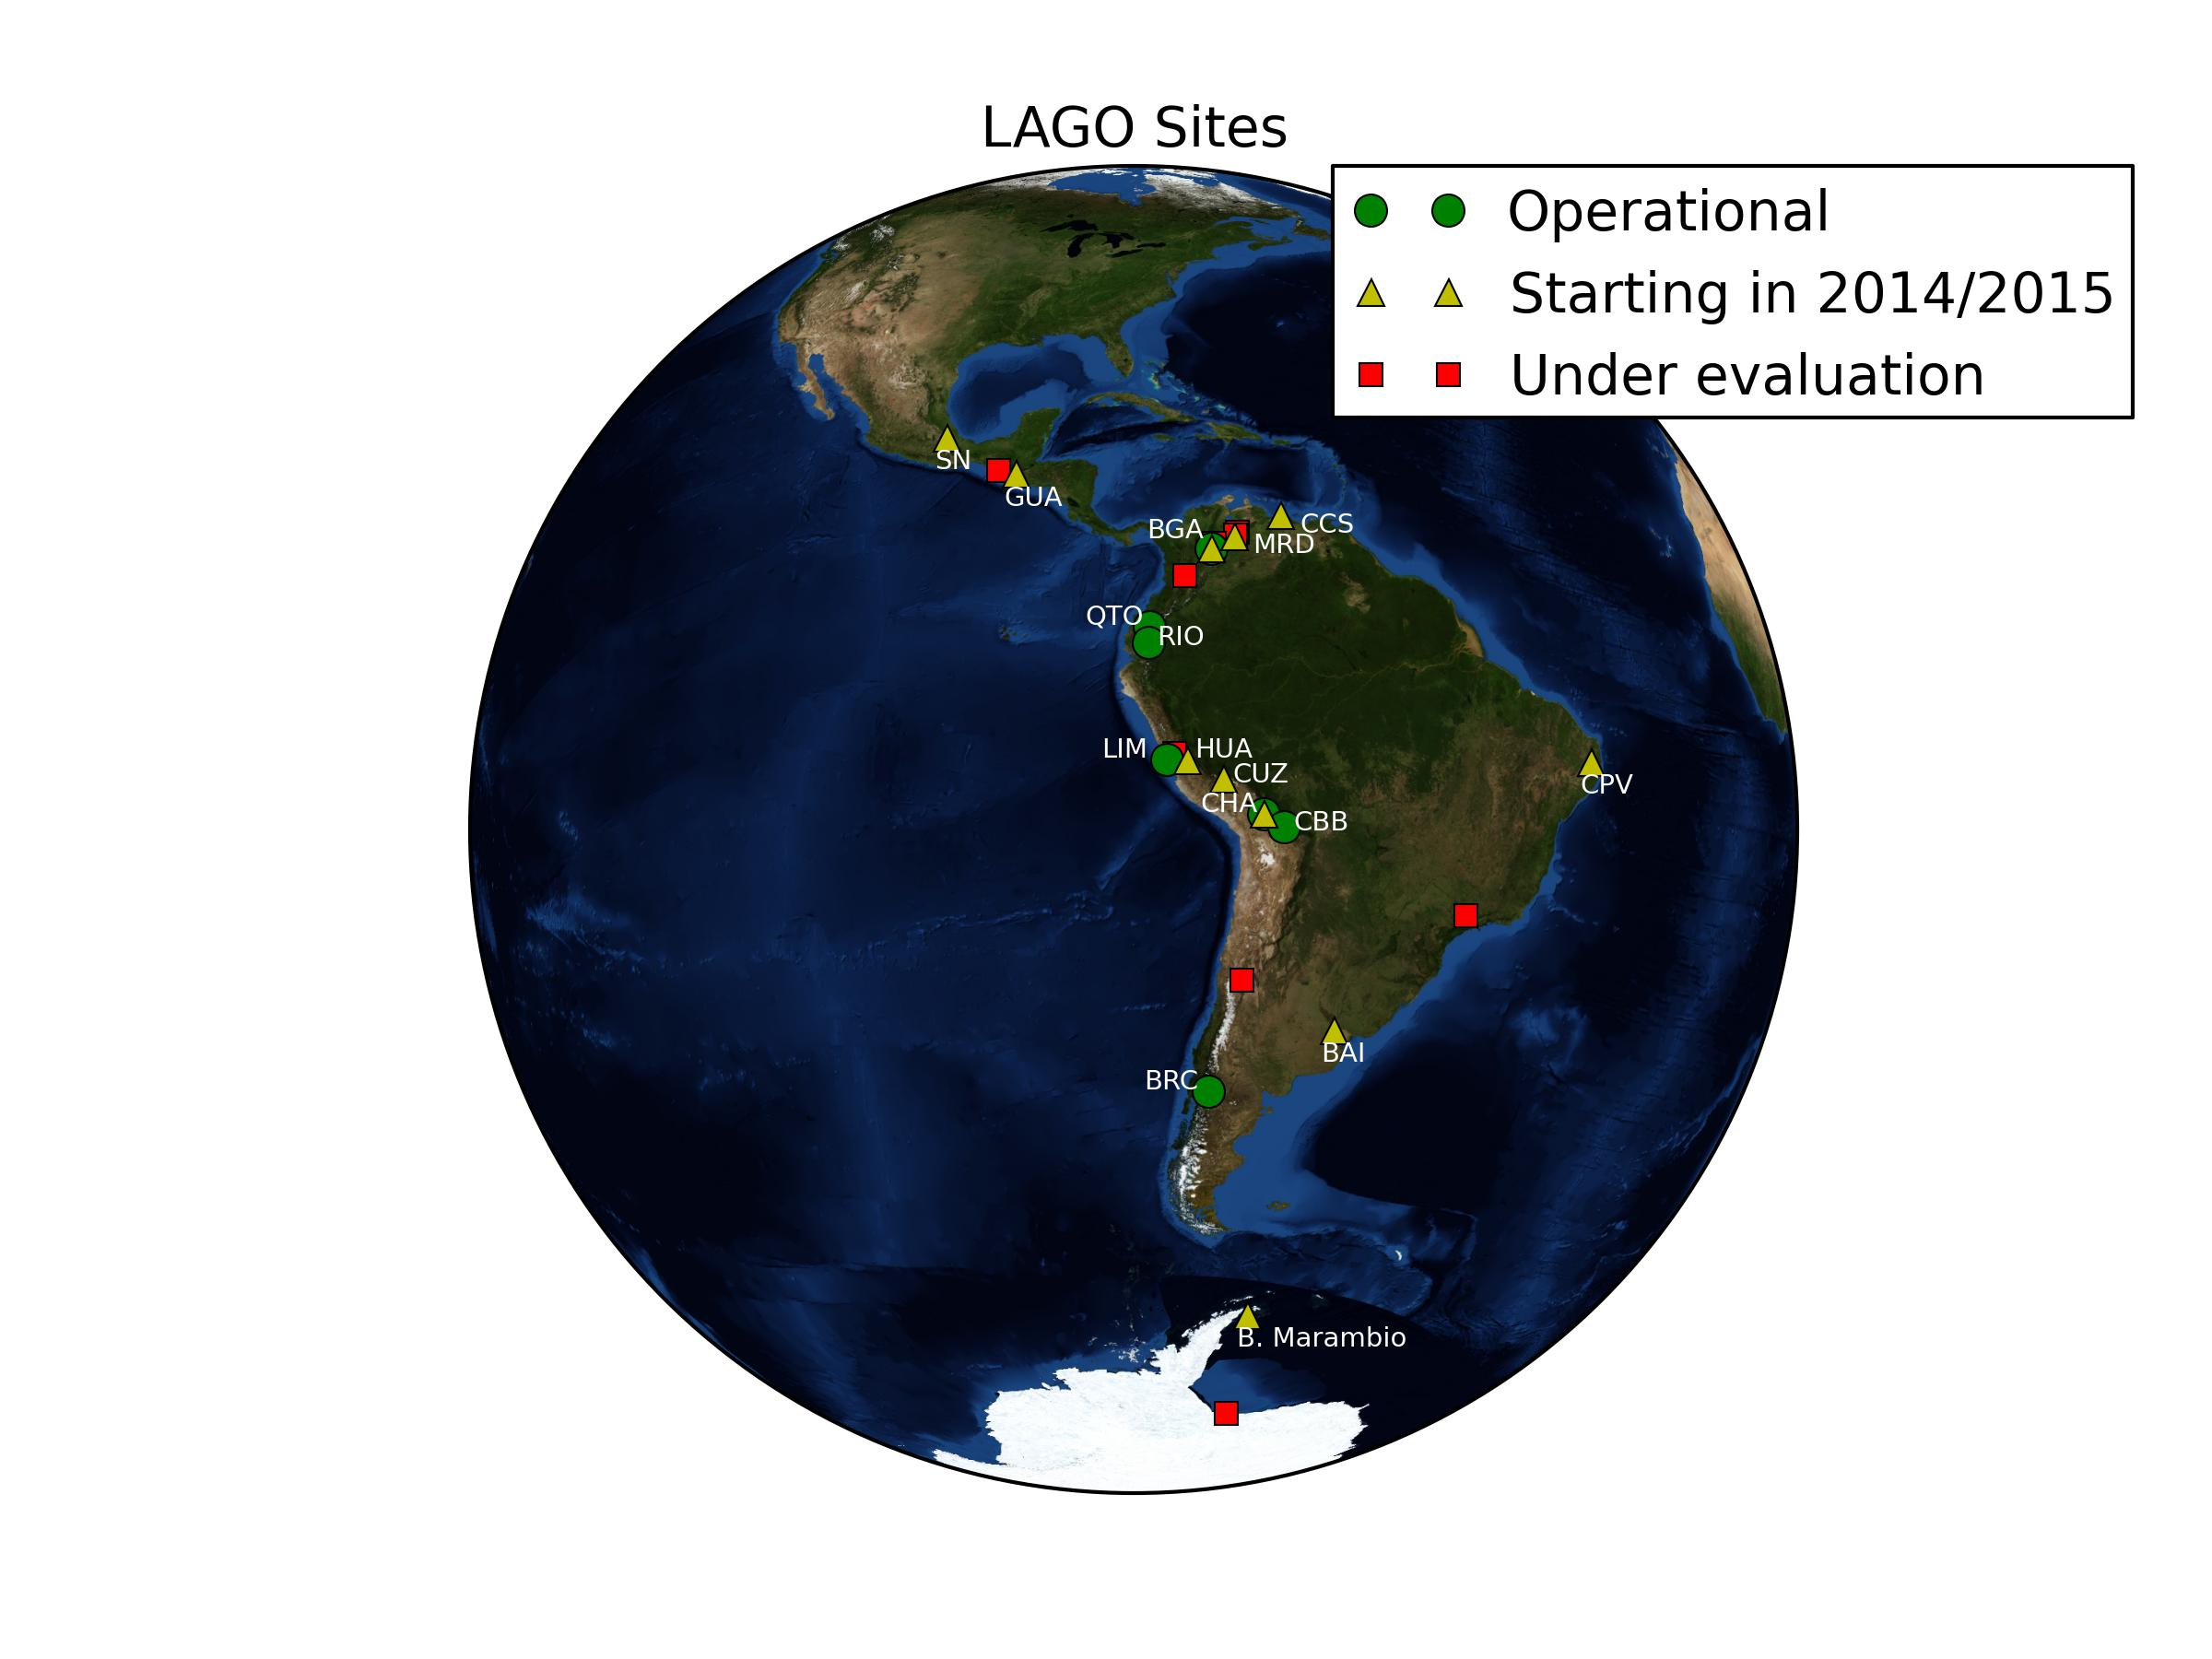
\includegraphics[width=.9\textwidth]{images/LagoMapa.jpg}
\caption{Google earth map showing all LAGO sites. For the color code label each
country that are in the LAGO collaboration. The markers shows if the detector
is operation at this day, is going to start measurements in the period
2014-2015 or the site is under evaluation to hold a WCD that will belong to the
LAGO network.} \label{fig:lago-map}
\end{figure}

To see the different sites, a compilation of the locations, detector size,
altitudes, rigidity cut off, latitude, longitude, and general observations are
made in table \ref{tab:locations}.

venezuela

\begin{table*}[!ht]
\begin{center}
\setlength{\tabcolsep}{0.2em}
\begin{tabular}{|c|c|c|c|c|c|c|c|c|}
\hline
\multirow{2}{*}{Country} & \multirow{2}{*}{Site} & Number of & Altitude & Altitude & Rigidity & Latitude &Longitude& \multirow{2}{*}{Observations}\\
 & & WCD & [m a.s.l.] & [g/cm$^2$] & cut off [GV] & [deg] & [deg] & \\
\hline
\hline
 \multirow{3}{*}{Argentina} &Bariloche &3&850 & & & 41.15 S& 71.30 W & \\
&Buenos Aires &1& 10& & 8.4$\pm$0.6 & 34.54 S & 58.44 W & \\
&Marambio &1& 200 & & & 64.24 S & 56.62 W & \\
\hline
Bolivia & Chacaltaya & 3 & 5240 & 530 & 12.5 & 16.35 S& 68.13 W & \\
\hline
Colombia & Bucaramanga & 1 & 956 &  & & 7.14 S& 73.12 W & \\
\hline
Ecuador & Chimborazo & 1 &  &  & & 1.81 S& 78.74 W & \\
\hline
Guatemala & Guatemala & 1 & 1490 &  & 8& 14.63 S& 90.59 W & \\
\hline
México & Sierra Negra & 4 & 4550 &  & 9& 18.16 S& 97.95 W & \\
\hline
\multirow{3}{*}{Perú} & Lima & 2  &150  &  & & 12.10 S& 77.02 W& \\
 & Cusco & 1& 3400 &  & & 13.52 S& 71.96 W& \\
 & Huancayo & 1& 3370 &  & & 12.04 S& 75.30 W& \\
\hline
 \multirow{3}{*}{Venezuela} &Caracas-UCV &1& 900& & 11.29 & 10.49 S & 66.89 W & \\
&Caracas-USB  &1& 1200& & 11.30 & 10.41 S & 66.88 W & \\
&M\'erida-ULA &1& 1893& &11.51 & 8.63 S & 71.15 W & \\
\hline
\end{tabular}
\caption{Table of the different locations of the LAGO sites.}
\label{tab:locations}
\end{center}
\end{table*}

